\Chapter{A Python eszközkészlet hatékonyságának vizsgálata}

\Section{A hatékonyság típusai}

A hatékonyság alatt általában a számítási hatékonyságot szokták érteni. Ez különösen igaz a numerikus számítások esetében. Nem szabad azonban figyelmen kívül hagyni a fejlesztéshez kapcsolódó további fontos jellemzőket sem. A NumPy a számítási műveletek jelentős részét alacsonyabb szinten (főként C nyelven) implementált egységek formájában tartalmazza. Emiatt annak számítási ideje jelentősen nem térhet el a natív implementációtól. Ezért a hatákonyság az alábbi szempontok kell, hogy fontosabb szerepet játszanak.
\begin{itemize}
\item A Python nyelv a számítási hatékonysággal szemben a program megírására, az elkészült programkód olvashatóságára helyezi a hangsúlyt. Annál hatékonyabbnak tekintjük tehát az eszközt, minél könnyebben értelmezhető és használható a benne készült program. Becsülhető például a programkód megírásához vagy megértéséhez, használatba vételéhez szükséges idővel.
\item A hatékonyságot segíti, hogy ha az elkészült algoritmusok minél egyszerűbben átvihetők más rendszerekre, tehát annál jobb, minél portábilisabb a megoldás. (A Python esetében ez az értelmező átvihetősége és elterjedtsége miatt adott.)
\item A hatékony használati módhoz hozzátartozik még az is, hogy a számítások bemenetét, a kapott eredményeket milyen könnyen lehet kezelni.
\item Fontos továbbá a megjelenítés módja, amelyet a Python a Matplotlib könyvtár segítségével kifejezetten támogat.
\end{itemize}

A következőkben különböző tématerületeket a numerikus módszerek tárgykörén belül, numerikus számítási módokat, a gyakorlatban és az oktatásban előforduló eseteket láthatunk, amely példaként szolgál arra, hogy a Python és az eszközkészlete milyen módon segíti a számítások elkészítésének, elvégzésének és ellenőrzésének a módját.

\Section{Hibaszámítás}

Amikor hibáról beszélünk akkor sok mindenre gondolhatunk, például egy
program írása közben kaphatunk futásidejű vagy fordítási idejű hibákat.
Nincs ez másképp a való életben sem, ott is lehet hiba ha megteszünk valamit vagy
ha éppen nem. Matematikai feladatok
esetében az alábbi hiba típusokról beszélhetünk.

\begin{itemize}
\item
  Modellhiba: amikor a valóságnak csak egy közelítését használjuk egy
  feladat matematikat alakjának a felírásához.
\item
  Mérési vagy öröklött hiba: amikor a modell adatai a valós pontos
  értékeknek csak valamilyen közelítő értékei, ezek általában a mérés
  pontosságától függnek
\item
  Műveleti és input hiba: ezek a hibák a számítógépen tárolt adatok
  számítógépen való ábrázolásánból adódó hibák. Ezek a számábrázolási
  hibák azért léphetnek fel, mivel a számítógépen a racionális számoknak
  is csak egy részhalmaza ábrázolható lebegő pontos aritmetikában. A
  műveletek elvégzésénél fel léphet kerekítés, túl- illetve
  alulcsordulás.
\item
  Képlethiba: amikor a végtelen eljárást véges számú lépés után
  leállítunk, közelítő eljárásokat alkalmazunk.
\end{itemize}

\SubSection{Számábrázolás}

\bigskip

\noindent\textbf{Egész számok}

\medskip

Számítógepen az egész számokat előjeles vagy előjel nélküli bináris
számként lehet ábrázolni, ezáltal jellemezhetőek a számjegyek számával.
Az egész számokat általában 2 vagy 4 byte-on tároljuk el 2-es, 10-es vagy
16-os számrendszerben. Ez az adott programozási nyelvtől függ. Az
egészekkel végzett aritmetikai műveletek általában gyorsabbak a lebegő pontos
számokkal végrehajtott aritmetikai műveleteknél, és ezáltal egy
algortimus lefutását fel tudja gyorsítani a használatuk. Használatuknál viszont
vigyázni kell arra, hogy tulajdonképpen maradékosztályokban dolgozunk.

\bigskip

\noindent\textbf{Lebegőpontos számok}

\medskip

Lebegő pontos számok esetében a számítógépek egy véges számhalmazt
ábrázolnak és a számításokat is ezekkel a számokkal végzik el \cite{ieee}.
Általában a lebegőpontos aritmetikát használják. Ennek nézzük meg a modelljét \aref{fig:ieee}. ábrán.

\begin{figure}[h!]
\centering
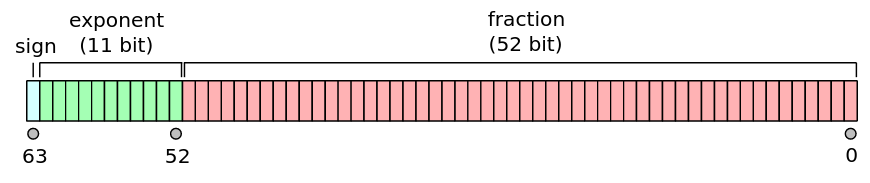
\includegraphics[width=\textwidth]{img/ieee.png}
\caption{Az egyszeres lebegőpontos számábrázolásnál a szám részeinek elrendezése IEEE 754-es szabvány szerint.}
\label{fig:ieee}
\end{figure}

A nem nulla lebegőpontos számok általános alakja a következő
\[
\pm a^k\left(\frac{m_1}{a}+\frac{m_2}{a^2}+\dots+\frac{m_t}{a^t}\right),
\]
ahol \(a > 1\) a számábrázolás alapja, \(\pm\) az előjel, \(t>1\) a számjegyek száma és \(k\in \mathbb{Z}\) a kitevő.

Az \(m_1\) számjegy normalizált, \((1\leq m_1 \leq a-1)\) ez garantálja
a az ábrázolás egyértelműségét. A többi
számjegy:\(1\leq m_i \leq a-1 \quad (i=2,3,\dots,t)\). A nulla az nem
normalizált tehát \(k=0, m_1=m_2=\dots=m_t=0\) és az előjele általában
\(+\). A számábrázolás alpaja itt is lehet 2, 10, 16 vagy akár más is,
átalában a programozási nyelven múlik melyiket használja. Pontosság
szempontjából a \(t=8\) az egyszeres pontosság, \(t=16\) a dupla pontosság.

A géptől és pontosságtól függően \(m\) tárolására \(32, 64\) vagy \(128\)
bit áll rendelkezésünkre (ez rendre \(4, 8, 16\) byte). Ezzel párhuzamosan
nő a \(k\) értékkészlete, és adott pontosság mellett:
\[
 L \leq k \leq U.
\]
A legnagyobb ábrázolható szám:
\[
M^\infty=a^U(1-a^-t)
\]
A legkissebb pedig:
\[
-M^\infty
\]
A lebegőpontos számok a \([-M^\infty,M^\infty]\)-beli számok diszkrét
(racionális) részhalmazát alkotják és ez a részhalmaz a nullára nézve
szimmetrikus. A nullához legközelebb eső lebegő pontos szám:
\(\varepsilon_0=a^{L-1}\) és az \(\varepsilon_0\)-hoz legközelebb eső
szám pedig: \(\varepsilon_0(1+a^{1-t})\).

A gép relatív pontossága vagy másképpen a gépi epszilon a
\(\varepsilon_1 = a^{1-t}\).

\SubSection{Klasszikus hibaanalízis}

Legyen \(A\) egy pontos érték, és legyen \(a\) ennek valamilyen
közelítése. A \(\Delta a=A-a\) mennyiséget a közelítés hibájának
nevezzük és a \(|\Delta a|=|A-a|\) pedig az abszolút hibájának. Azt a
\(\delta a\) értéket pedig abszolút hibakorlátnak nevezzük amelyre
fenáll, hogy \(|A-a|=|\Delta a| \leq \delta a\).

Az \(A\) szam valamilyen közelítő értékének a relatív hibája pedig a
\(\frac {\delta a} {A}\) mennyiség.

Az additív műveletek abszolút hibákorlátja pedig a következőek:
\[
\delta(a+b) \leq \delta a+ \delta b, \quad
\delta(a-b) \leq \delta a+ \delta b.
\]

Az multiplikatív műveletek abszolút hibákorlátjai:
\[
\delta(ab) \approx |a|\delta b +|b| \delta a, \quad
\delta(a/b) \approx  \frac {|a|\delta b +|b| \delta a}{|b|^2}.
\]

Az aritmetikai műveletek relatív hibakorlátjai a következőek, feltéve
hogy a nevező sehol sem nulla és az additív műveleteknél az operandusok
megegyező előjelűek:

\[
\frac{\delta(a+b)} {|a+b|} =  \max\left( \frac{\delta a}{|a|}, \frac{\delta b}{|b|} \right), \quad
\frac{\delta(a-b)} {|a-b|} = \frac{\delta a + \delta b} {|a-b|},
\]

\[
\frac{\delta(ab)} {|ab|} \approx \frac{\delta a}{|a|} + \frac{\delta b}{|b|}, \quad
\frac{\delta(\frac {a}{b})} {|\frac {a}{b}|} \approx \frac{\delta a}{|a|} + \frac{\delta b}{|b|}.
\]

\Section{Vektor és mátrix műveletek}

\SubSection{Vektorok}

Pythonban a \emph{NumPy} csomag használatával könnyedén definiálhatunk
vektorokat és mátrixokat. Ahhoz, hogy használhassuk előtte telepíteni
kell majd be kell a \texttt{pip} csomagkezelővel, majd az alábbi módon lehet
importálni:
\begin{python}
import numpy as np
\end{python}

Ez a szintaktikája Python-ban egy csomag inportálásának. Az \texttt{as}
operátor után aliast adhatunk a csomagnak, így megkönyítve a
használatát. Alias megadása nem kötelező.
Ez esetben \texttt{np}-vel tudunk hivatkozni a \emph{NumPy} csomagra. A csomagból az \texttt{array} metódus segítségével hozhatunk
létre vektorokat, például
\begin{python}
v1 = np.array([1, 2, 3])
v2 = np.array([3, 2, 1])
v3 = np.array([5, 3, 1, 6])
\end{python}

    Üres vektort a következőképpen készíthetünk: az \texttt{empty}
metódusban meg kell adni szögletes zárójelek között egy dimenziót
(például: \texttt{{[}1,\ 3{]}} ez azt jelenti 1 sort és 3 oszlopot
szeretnénk), és esetlegesen megadhatunk neki egy adattípust, hogy milyen
adatokkal szeretnénk feltölteni.

    Itt főleg valmilyen numerikus adattípusra kell gondolni, hisz ezekkel
tudjuk elvégezni a vektor és mátrix műveleteket. Haszálhatjuk a Python
beépített típusait, mint az \texttt{int} vagy a \texttt{float}, de
használhatjuk a \emph{NumPy}-ban definiált kiegészített változatokat
amivel megadhatjuk azt például, hogy hány bájton tároljuk az adott
számot. Esetlegesen megadhatunk stringet és bool típust is ha szükség
van rá.

Az \texttt{empty} nem feltétlenül 0-ákkal tölti fel a vektort hanem valamilyen
memória szeméttel.
\begin{python}
v4 = np.empty([1, 3])
\end{python}
Ennek az oka nagyon egyszerű: így gyorsabb, mint ha
nullázná az elemeket, de ha 0-ákkal szeretnénk feltölteni használhatjuk
a \texttt{zeros} metódust mely hasonló képpen működik mint az
\texttt{empty}:
\begin{python}
v5 = np.zeros([1, 3])
\end{python}
    1-esekkel is feltölthetjük ehez a \texttt{ones}metódust használhatjuk:
\begin{python}
v6 = np.ones([1, 3])
\end{python}
    Létrehozhatunk egy bizonyos értékkel vagy pszeudóvéletlen (random)
számokkal feltöltött vektorokat is :
\begin{python}
v7 = np.random.rand(1, 3)
v8 = np.full([1, 3], "aaa")
\end{python}
Utóbbiak a következő értékeket tartalmazzák:
\begin{verbatim}
[[0.22541693 0.47521003 0.90312494]]
[['aaa' 'aaa' 'aaa']]
\end{verbatim}
    A fent létrehozott \texttt{v1}, \texttt{v2}, \texttt{v3} vektorainkal
már egyszerűen elvégezhetőek a vektor műveletek, mint például az
összeadás, kivonás, vektoriális, skaláris szorzás és konstanssal való szorzás:
\begin{python}
v1 + v2
v1 - v2
np.outer(v1, v2)
np.inner(v1, v2)
v1 * 3
\end{python}
Amennyiben egyszerűen a összeszorozzuk a két vektort akkor a megfelelő hely lévő
tagokat szorozaz össze:
\begin{python}
v1 * v2
\end{python}
Transzponálhatjuk is a vektorainkat a \texttt{transpose} metódussal bár
vektorok esetén itt nem látványos:
\begin{python}
v3.transpose()
\end{python}
Komolyabb műveletek mint a vektor normák kiszámítása is egyszerű. Vegyük
először az 1-es normát:
\begin{python}
np.linalg.norm(v1, 1)
\end{python}
Itt használtuk a numpy \texttt{linalg} csomagját melyben előre
definiálva vannak a különbőző lineáris algebrához tartozó műveletek,
módszerek. Most nézzük a 2-es és a végtelen normát:
\begin{python}
np.linalg.norm(v1, 2)
np.linalg.norm(v1, np.inf)
\end{python}
    Mind itt a vektorműveleteknél, és majd a mátrix műveleteknél sem árt
figyelni, hogy megfelelő dimenziójú vektorokat, mátrixokat adjunk meg a
műveletekhez, különben könnyen hibát vagy helytelen eredményt kaphatunk.

\SubSection{Mátrixok}

A Mátrixok létrehozása is többféleképpen történhet, hasonlóképpen mint a
vektoroknál. Legegyszerűbb módszer az, ha megadjuk mi, hogy milyen
mátrixot szeretnénk vagy képezhetjük vektorokból is, estleg a fent
megismert \texttt{empty,\ zeros,\ ones,\ random.rand,\ full}
metódusoknak megadjuk a nekünk megfelelő dimenziókat.
\begin{python}
m1 = np.matrix([[1, 2, 4], [2, 3, 4]])
m2 = np.matrix([[1, 2, 8], [2, 3, 9]])
m3 = np.matrix([[1, 2], [2, 3], [4, 5]])
m4 = np.matrix([[1, 2], [3, 4]])
\end{python}
Tartományok segítségével is létrehozhatunk mátrixokat.
\begin{python}
m = np.arange(16.0)
m = np.arange(16.0).reshape(4, 4)
\end{python}
    A \texttt{reshape}-nél vigyázni kell, hogy pontosan akkora elemszámú
mátrixot adjunk meg mint amekkora a mostani mátrixunké, különben hibát
kapunk. Amennyiben mégis kisebb vagy nagyobb mátrixot szeretnénk használni, át kell másolni az elemeket egyik mátrixból a másikba.
    Az \texttt{eye} metódus segítségével képezhetünk \(n*n\)-es
egységmátrixot, paraméterként a dimenziót kell megadnunk:
\begin{python}
m = np.eye(3)
\end{python}
amely a következő mátrixot hozza létre:
\begin{verbatim}
[[1. 0. 0.]
 [0. 1. 0.]
 [0. 0. 1.]]
\end{verbatim}
    A vektorokhoz hasonlóan adhatjuk meg a mátrix műveleteket is, mint az
összeadást, kivonást, szorzást, normákat:
\begin{python}
m1 + m2
m1 - m2
m1 * m3
np.linalg.norm(m1, 'fro')
np.linalg.norm(m1, np.inf)
np.linalg.norm(m1, 1)
np.linalg.norm(m1, 2)
\end{python}
A transzponálás is hasonlóan működik:
\begin{python}
m3.transpose()
\end{python}
    Egy négyzetes mátrix determinánsát és inverzét is egyszerűen és gyorsan
kiszámíthatjuk a következő formában:
\begin{python}
np.linalg.det(m4)
np.linalg.inv(m4)
\end{python}
    Egy elemet az \texttt{item} metódussal tudunk kiválasztani, de figyelni
kell, mert az indexelés 0-tól kezdődik:
\begin{python}
print("Az m3 2. sor 1. eleme", m3.item(1, 0))
\end{python}
    A mátrixokat feldarabolhatjuk a \texttt{hsplit} és \texttt{vsplit}
metúdusok segítségével. A \texttt{hsplit} oszlopok mentén, míg a
\texttt{vsplit} sorok mentén vágja el a megadott mátrixot:
\begin{python}
np.hsplit(m, 2)
np.vsplit(m, 2)
\end{python}
    Használhatjuk vágásra az \texttt{{[}{]}} operátorokat is, ha csak egy
paramétert adunk meg neki akkor az adott indexű sort kapjuk vissza, ha
használjuk a \texttt{:} operátort akkor megadhatunk neki intervallumot
is, hogy hanyadik sornál kezdje, megadhatunk neki lépésközt is illetve
részeket is kivághatunk egy adott mátrixból, például
\begin{python}
m[1:3]
m[:, 1:3]
m[1:3, 1:3]
\end{python}
    Ha adunk meg neki lépésközt, akkor az az utolsó paraméter. Például az egész
mátrix minden párátlan számú sorának és oszlopának a közös elemei:
\begin{python}
m[0:4:2, 0:4:2]
\end{python}

\Section{Mátrix felbontások}

\SubSection{LU felbontás}
    
    Mátrixok LU felbontásásval kinyerhetjük a felső-  és alsóháromszög
mátrixot. Pythonban erre használható a\texttt{Scipy.linalg.lu} metódus
ami a \texttt{SciPy} tudományos csomagban találhatunk meg ami egy
kiegészítése tulajdon képpen a \texttt{NumPy}-nak. Először telepíteni és
importálni kell ezt a csomagot és utána használatba lehet venni. Az
\texttt{lu} metódus végeredményként visszaadja az alsó-, felső- és a
permutáció mátrixokat.
\begin{python}
import scipy as sp
from scipy.linalg import lu
m =np.arange(16.0).reshape(4, 4)
P, L, U = sp.linalg.lu(m)
\end{python}

\SubSection{Cholesky felbontás}

    A Cholesky féle felbontásra is találunk beépített metódust a
\texttt{Numpy}-ban \texttt{cholesky} néven a \texttt{linalg} csomagban.
Cholesky felbontásnál vigyázni kell hogy a mátrixunk szimmetrikus legyen
és pozitív definit ellenben hibaüzenetet kapunk. Ugyan ez megtalálható a
\texttt{SciPy} csomagban is és a különbség az, hogy a \texttt{NumPy}-ban
lévő metódus az alsó-, addig a \texttt{SciPy}-ban lévő a felsőháromszög
mátrixot számolja:
\begin{python}
m =np.arange(16.0).reshape(4, 4)
L=np.linalg.cholesky(m)
\end{python}
    A fenti kód hibát eredményezett, mert a megadott mátrix nem volt pozitív
definit. A következő példában már pozitív definit mátrix szerepel:
\begin{python}
m = np.array([[2, -1, 0], [-1, 2, -1], [0, -1, 2]])
L = np.linalg.cholesky(m)
L = sp.linalg.cholesky(m)
\end{python}
Természetesen megírhatjuk a saját felbontó függvéníünket is:
\begin{python}
import numpy as np
import scipy as sp

def cholesky(M, dimensions):
    P, L, U = sp.linalg.lu(M)
    k = 0
    while k<dimensions:
        j = 0
        s = 0
        while j < k - 1:
            s = L[k, j] * L[k, j]
            j += 1
        L[k, k] = np.sqrt(M[k, k] - sum)
        i = k + 1
        while i < dimensions:
            j = 0
            s = 0
            while j < k - 1:
                s = L[i, j] * L[k, j]
                j += 1
            L[i, k] = (M[i, k] - s) / L[k, k]
            i += 1
        k += 1
    return L

m = np.array([[2, -1, 0], [-1, 2, -1], [0, -1, 2]])
dimension = 3
l = cholesky(m, dimension)
\end{python}
Ahogy láthajuk a metódus megadja egy közelítő megoldását a cholesky
felbontásnak.

\Section{Lineáris egyenletrendszerek}

\SubSection{Általánosan a lineáris egyenletredszerekről}

    A lineáris egyenletrendszer egy többismeretlenes egyenletrendszer
melyben az ismeretlenek az első hatványon vannak.

    Egy \(n\) egyenlet és \(m\) változó esetén az egyenletrendszer általános
alakja a következő:

\begin{align*}
x_{1,1} + x_{1,2} + \dots + x_{1,m} &= b_{1}\\
x_{2,1} + x_{2,2} + \dots + x_{2,m} &= b_{2}\\
\vdots\\
x_{i,1} + x_{i,2} + \dots + x_{i,m} &= b_{i}\\
\vdots\\
x_{n,1} + x_{n,2} + \dots + x_{n,m} &= b_{n}\\
\end{align*}
Azt mondjuk, hogy az egyenlet rendszer alulhatárolt, hogy ha \(n < m\) és
túlhatárolt, hogy ha \(n>m\). Négyzetesnek nevezzük, ha \(m = n\). Az
egyenletrendszer geometriai tartalmát az alábbi módon írhatjuk le:
    Az \(R^n\) euklideszi tér \(d\in R^n\) normálvektorú és \(x_0 \in R^n\)
ponton átmenő hipersíkját az
\[
(x - x_0)^Td=0
\]
egyenletet kielégítő \(x \in R^n\) pontok határozzák meg.

Az \(Ax=b\) egyenletrendszert felírhatjuk ilyen formában is:
\begin{align*} 
a_{1}^Tx &= b_1,\\
a_{2}^Tx &= b_2,\\
\vdots\\
a_{n}^Tx &= b_n,\\
\end{align*}
ahol \(a_{i}^T={a_{i1}, \dots a_{im}}\).
Innen láthatjuk, hogy az egyenletrendszer megoldása az \(m\) hipersík
közös része, ennek megfelelően 3 megoldás lehetséges: nincs megoldás, pontosan egy megoldás van vagy végtelen sok megoldás van.
Ha az \(Ax=b\) egyenletrendszernek legalább egy megoldása létezik
konzisztensnek nevezzük. Ha nem létezik egyetlen megoldása sem, akkor az
egyenletrendszer inkonzisztens.

\subsection{Lineáris egyenletrendszerek megoldása Python-ban}

Egy egyenletrendszert megoldani Python-ban nem nehéz. A \texttt{NumPy}
tartalmazza a \texttt{solve} metódust mellyel könnyedén megoldható
egy-egy lineáris egyenletrendszer. A \texttt{solve} a \texttt{NumPy}
linalg csomagjában található, paramáterként várja az \(A\)
együtthatómátrixot és a \(b\) megoldásvektort. Nézzük is meg!
Vegyünk először egy egyszerű egyenletrendszert, mint a következő:
\begin{align*}
    2x_1 + 9x_2 + 8x_3 + 7x_4 &= 7, \\
    3x_1 - 2x_2 + 6x_3 + 4x_4 &= 4, \\
    5x_1 + 8x_2 + 4x_3 + 7x_4 &= 2, \\
    6x_1 + 9x_2 + 10x_3 + 2x_4 &= 6.
\end{align*}
Importáljuk a \texttt{numpy} és a \texttt{time} csomagot:
\begin{python}
import numpy as np
import time
\end{python}
Miután ezzel megvagyunk hozzuk létre az együttható métrixunkat és a
megoldás vektorunkat:
\begin{python}
a = np.array([
    [2,  9, 8,  7],
    [3, -2, 6,  4],
    [5,  8, 4,  7],
    [6,  9, 10, 2]])
b = np.array([7, 4, 2, 6])
\end{python}
Használjuk a \texttt{solve} metódust
\begin{python}
start = time.time()
import numpy as np
x_solve = np.linalg.solve(a, b)
print("Eredmeny:")
print(x_solve)
time_solve=time.time() - start
print("\nFutasi ido:\n")
print(time_solve)
\end{python}
    A solve az Intel Math Kernel Library-ben megtalálható LAPACK \texttt{gesv} rutint
használja.
A futás időt is kiírja a program, hogy később össze lehessen vetni a
beépített és az általam implementált algoritmust. Az \texttt{allclose}
és \texttt{dot} metódusok segítségével pedig le is ellenőrízhetjük az
eredményt.
\begin{python}
np.allclose(np.dot(a, x_solve), b)
\end{python}       
    Ilyen egyszerű az egész, de ha nem szeretnénk az előre megírt metódust
alkalmazni akkor definiálhatunk saját magunk is nekünk tetsző megoldó
metódust is. Például implementálhatjuk a Gauss módszert is. Ám mielőtt
ezt megnéznénk vessünk egy pillantást a ciklusokra Python-ban csak, hogy
érthető legyen a kód.

    Egy lineáris egyenletrendszer csak akkor megoldható ha az $A$ matrixunk
rangja megyegyezik az $[A, b]$ mátrix rangjával. Ilyenkor az
egyenletrendszerünknek pontosan egy megoldása van. Ezt Python-ban a
következőképpen tudjuk ellenőrizni:
\begin{python}
print("A matrix rangja:")
print(np.linalg.matrix_rank(a))
c = np.column_stack((a, b.transpose()))
print("[A, b] matrix rangja:")
print(np.linalg.matrix_rank(c))
\end{python}
Ennek az eredményéből látható lesz, hogy a két rang megegyezik, ezáltal megoldható az itt látható
egyenlet rendszer.

A Gauss módszer elkészítése kapcsán bemutathatók a Python nyelv vezérlési szerkezetei.
Python-ban is megtalálható a \texttt{for} és a \texttt{while} ciklus. A
\texttt{for} végig iterál egy iterálható objektumon ami pythonban lehet
egy tömb, string vagy az általunk kreált iterálható struktúra.
\begin{python}
s = "string"
tomb = [1, 3, 5]
collection = ["string", 8, 'a']

for i in s:
    print(i)

for i in tomb:
    print(i)

for i in collection:
    print(i)
\end{python}
    Ha klasszikus értelemben szeretnénk használni (tehát egy ciklus változót
léptetni egy kezdő értéktől egy végértékig) használnunk kell a
\texttt{range} metódust mely generál egy tömböt a megadott paraméterek
alapján. Három paramétere van, az első a kezdő érték, a második a
végérték és a harmadik a lépésköz. A \texttt{range} esetében figyelni
kell, mert a végéertékig generálja a számokat ezért a végérték nem
szerepel az általa vissza adott iterálható példányban:
\begin{python}
x = range(1, 4)

for i in x: 
    print(i)

for i in range(1, 50, 2):
    print(i)
\end{python}
    A \texttt{while} működése nem tér el a többi általános célú programozási
nyelvekben megszokottól. Amíg a megadott feltételünk igaz addig maradunk a
ciklusban, például
\begin{python}
x = 0
while x < 10:
    x += 1
\end{python}
    Nézzük még meg az \texttt{if} elágazást is mely megvizsgál egy logikai
kifejezést és annak értéke szerint ágaztatja el a programot.
\begin{python}
if True:
    print("igaz")
    
if False:
    print("igaz")
else:
    print("hamis")
    
if 2 + 2 == 4:
    print("two plus two is four")
\end{python}
Ezen ismeretek birtokában már belekezdhetünk a Gauss módszer implementációjának vizsgálatába:
\begin{python}
import numpy as np
import time

def gauss(a, b, dimension):
    l = np.zeros([dimension, dimension])
    x = np.zeros([dimension])

    for k in range(0, dimension - 1):
        for i in range(k + 1, dimension):
            l[i, k] = a[i, k] / a[k, k]
            b[i] = b[i] - (l[i, k] * b[k])
            for j in range(k, dimension):
                a[i, j] = a[i, j] - (l[i, k] * a[k, j])

    x[dimension - 1] = b[dimension - 1] / a[dimension - 1, dimension - 1]
        
    for i in range(dimension - 1, -1, -1):
        s=0
        for j in range(i + 1, dimension):
            s = s + a[i, j] * x[j]
            x[i] = (b[i] - s)/a[i, i]
    return(x)

start = time.time()
a = np.array([
    [2,  9,  8, 7],
    [3, -2,  6, 4],
    [5,  8,  4, 7],
    [6,  9, 10, 2]])
b = np.array([7, 4, 2, 6])
dimension = 4
x_g = gauss(a, b, dimension)
print("Eredmeny:\n")
print(x_g)
time_gauss = time.time() - start
print("\nFutasi ido:\n")
print(time_gauss)
\end{python}
A futtatás után láthatóvá válik, hogy időben elég közel van a numpy-ban lévő megoldáshoz. De
nem kapunk olyan pontos eredményt.

    Tegyünk most kis kitérőt a számítási munkára. Ezt valahogyan mérni kell,
hogy megtudjuk adni egyes algoritmusoknak a műveletigényét, és ennek a
mértékegysége a flop. Egy régi flop az a számítási munk ami az
\(s = s + x*y\) művelet (egy összeadés és egy szorzás) elvégzéséhez kell, 1
új flopp pedig az a számítási munka mely egyetlen művelet (mindegy az
hogy additív vagy multiplikatív) elvégzéséhez szükséges. Az új flop
bevezetését az indokolta, hogy a mai számítógépeken a multiplikatív és
az additív műveletek elvégzéséhez szükséges idő azonosnak tekinthető.

    A gauss módszer $\dfrac{n^3}{3} + O(n^2)$ addítív és ugyanennyi
multiplikatív műveletet igényel, így a művelet igénye:\(\dfrac {n^3}{3}+
O(n^2) \) régi flop és \(\dfrac {2n^3}{3}+ O(n^2) \) új flop.

\bigskip

\noindent\textbf{Főelem kiválasztás}

\medskip

    A fenti algoritmus csak olyan mátrixokat képes megoldani amikben egyik
együttható sem nulla. Hogy képes legyen rá ki kell egészíteni főelem
kiválasztással. A főelem kiválasztás azt jelenti, hogy a sorokat úgy
cseréljük fel, hogy az aktuális pivot elemünk ne legyen nulla. A
főelemkiválasztás lehet részleges vagy teljes. Részleges főelem
kiválasztásnál a \(k\)-adik lépésben megkeressük a \(k\)-adik oszlop
elemei közül a maximális abszolút értékű \(a_{ik}\) együtthatót és ez az
\(j\)-edik sorban van akkor megcseréljük a \(j\)-edik és a \(k\)-adik
sort. Ezzel fogunk majd találkozni a gauss-Jordan módszer
implementációjánál. A teljes főelem kiválasztás során pedig a \(k\)-adik
lépésben megkeressük a mátrixban szereplő értékek közül a maximális
abszolút értékűt és ha ez a \(a_{ij}\) akkor a \(k\)-adik sort
felcseréljük az \(i\)-edikkel és a \(k\)-adik oszlopot is felcseréljük a
\(j\)-edikkel.

\bigskip

\noindent\textbf{Gauss-Jordan módszer}

\medskip

    Egy másik lehetséges módszer az egyenletrendszerek megoldására a
Gauss-Jordan módszer. Ezt implementálhatjuk mi magunk is, de én most egy
másik csomagot a SymPy-t fogom segítségül hívni. Első lépésnek vegyük az
\(A\) mátrixunkat és a \(b\) vektorunkat, majd használjuk az A mátrixra
definiált \texttt{gauss\_jordan\_solve} mmetódust melynek paraméterként
a \(b\) vektort adjuk meg. A metódus két visszatérési értéke a megoldás
és a mátrix.
\begin{python}
from sympy import Matrix

start = time.time()
A = Matrix([
    [2,  9,  8, 7],
    [3, -2,  6, 4],
    [5,  8,  4, 7],
    [6,  9, 10, 2]])
b = Matrix([7, 4, 2, 6])
sol, params = A.gauss_jordan_solve(b)

n, m = sol.shape
x_gj= np.zeros(n)
for i in range(0, n):
    x_gj[i]= sol[i]

time_gauss_jordan = time.time() - start
print("Eredmeny:")
print(x_gj)
print("Futasi ido:")
print(time_gauss_jordan)
\end{python}
    Fontos figyelembe venni, hogy a \texttt{Matrix} nem kompatibilis az \texttt{np.array}-el, így az értékeket
nekünk kell áthelyezni.

    Van egy 4. módszer is a lineáris egyenlet rendszer megoldására a
\texttt{scipy} csomagban, ami az LU-faktorizáción alapul. A metódus neve
pedig \texttt{lu\_solve} és az alábbi módon lehet használni:
\begin{python}
from scipy.linalg import lu_factor, lu_solve

start=time.time()
A = Matrix([
    [2,  9,  8, 7],
    [3, -2,  6, 4],
    [5,  8,  4, 7],
    [6,  9, 10, 2]])
b = Matrix([7, 4, 2, 6])
lu, piv = lu_factor(A)
x_lu = lu_solve((lu, piv), b)

time_lu = time.time() - start
print("Eredmeny:")
print(x_lu)
print("futasi ido:")
print(time_lu)
\end{python}
A \texttt{pandas} függvénykönyvtár segítségével összesítő táblázatot is készíthetünk, amely eredményét \aref{fig:leq-summary}. ábrán láthatjuk.

\begin{figure}[h!]
\centering
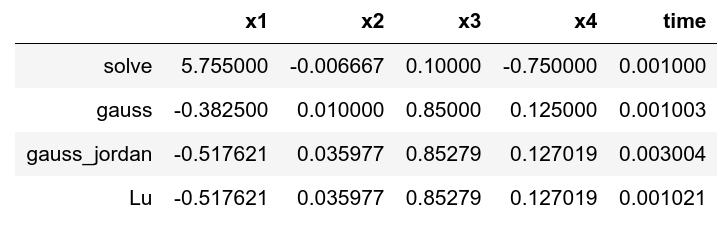
\includegraphics[width=\textwidth]{img/leq_summary.png}
\caption{Az egyenletrendszer megoldó módszerek eredményeinek összesítése és megjelenítése Pandas segítségével.}
\label{fig:leq-summary}
\end{figure}

\Section{Interpolációk}

    Az interpolációk alapfeladata az, hogy egy \(f(x)\) függvény felvett
értékeit különböző \(x_1, x_2 x_3 \dots x_n\) pontokban ismerjük az
\([a,b](a=x_1, b=x_n)\) intervallumban és magát az \(f\) függvényt
szeretnénk közelíteni egy könnyen számolható \(h(x)\) függvénnyel,
amelyre fenáll, hogy \(f(x_i)=h(x_i)\). Az \({x_i}, i=1, \ldots, n\) pontokat
interpolációs alappontoknak, a feltételt interpolációs feltételnek
nevezzük. Az interpolációs feltétel teljesülése esetén azt reméljük,
hogy az interpoláló \(h(x)\) függvény jól közelíti az \(f(x)\) függvényt
az \([x_i, x_i + 1]\) intervallumokban. Itt a Lagrange, Hermit és Spline
interpolációkról fogok elsősorban írni.

    Legegyszerűbben interpolációt az \texttt{interp1d} függvénnyel tudunk
végre hajtani. Ez a módszer nem kér csak \(x, y\) értékeket és az
interpoláció módját. A metódus a \texttt{scipy} csomag \texttt{interpolate} alcsomagjában található
meg.
A következő kódrészletben egy ezzel készített példa látható.
\begin{python}
from scipy.interpolate import interp1d
import matplotlib.pyplot as plt
from matplotlib.pyplot import figure

x = np.linspace(0, 10, num=7, endpoint=True)
y = np.cos(-x**2/12)
f = interp1d(x, y)
f2 = interp1d(x, y, kind='cubic')
f3 = interp1d(x, y, kind='quadratic')
xnew = np.linspace(0, 10, num=200, endpoint=True)

plt.figure(figsize=(18.5, 10.5))
plt.plot(x, y, 'o',
    xnew, f(xnew), '-', xnew, f2(xnew), '--', xnew, f3(xnew), '.-')
plt.legend(['eredeti y ertekek', 'linearis', 'kobos', 'kvadratikus'],
    loc='best')
plt.show()
\end{python}
A programrész kimenetét \aref{fig:interpolate}. ábrán tekinthetjük meg.

\begin{figure}[h!]
\centering
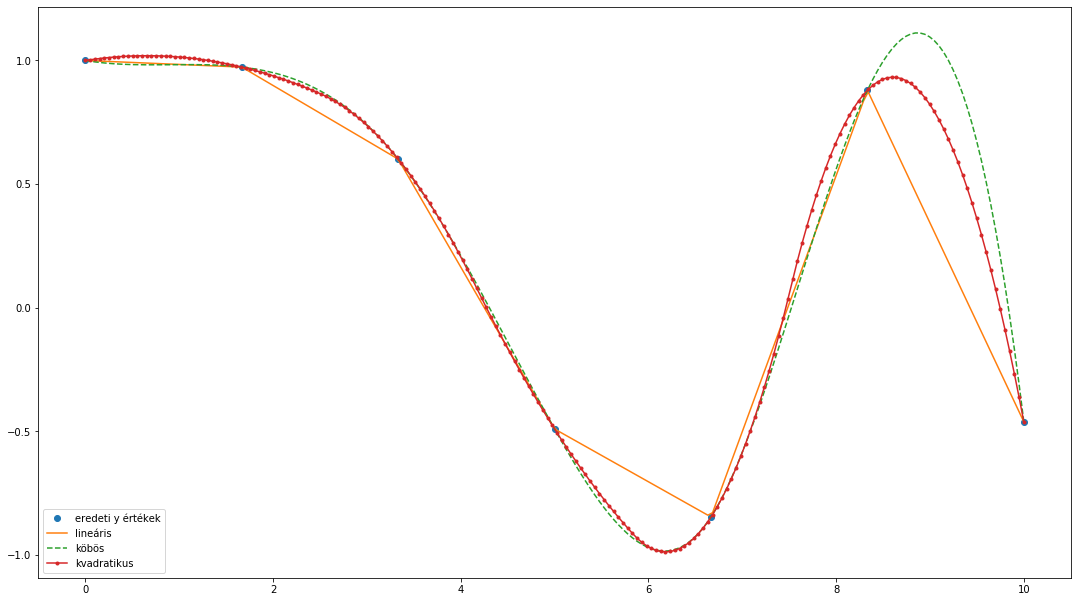
\includegraphics[width=\textwidth]{img/interpolate.png}
\caption{Példa az interpolált pontok számítására és megjelenítésére.}
\label{fig:interpolate}
\end{figure}
    
    Látható, hogy az \texttt{interp1d} egy függvénnyel tér vissza, aminek csak meg
kell adnunk az \(x\) értékeinket és vissza adja az eredményt. Ezek
használhatóak a legkönnyebben Python-ban. fontos, hogy miután elvégeztük
az interpolációt adott pontokra, a függvénynek azonos intervallumon de
több alpontot tartalmazó tömböt adjunk át kirajzolásnál, hogy szépen és
pontosan rajzolja ki a közelítő függvényt.

    Míg az \texttt{interp1d} \(y = f(x)\) típusú függvényeket interpolál, addig
ennek a metódusnak a párja az \texttt{interp2d} már az \(z = f(x, y)\)
tipusú egyenleteket tudja közelíteni. használata az
\texttt{interp1d}-hez hasonló, például
\begin{python}
import numpy as np
from scipy import interpolate
import matplotlib.pyplot as plt
from matplotlib import figure

x = np.arange(-8, 8, 0.25)
y = np.arange(-8, 8, 0.25)
xx, yy = np.meshgrid(x, y)
z = np.sin(xx**2 + yy**2)
f = interpolate.interp2d(x, y, z, kind='cubic')

xnew = np.arange(-8, 8, 1e-2)
ynew = np.arange(-8, 8, 1e-2)
znew = f(xnew, ynew)

plt.figure(figsize=(18.5, 10.5))
plt.plot(x, z[0, :], 'ro', xnew, znew[0, :], 'b--')
plt.legend(["eredeti pontok", "interpolalo fv."])
plt.show()
\end{python}
A program kimenetét \aref{fig:cubic}. ábrán láthatjuk.

\begin{figure}[h!]
\centering
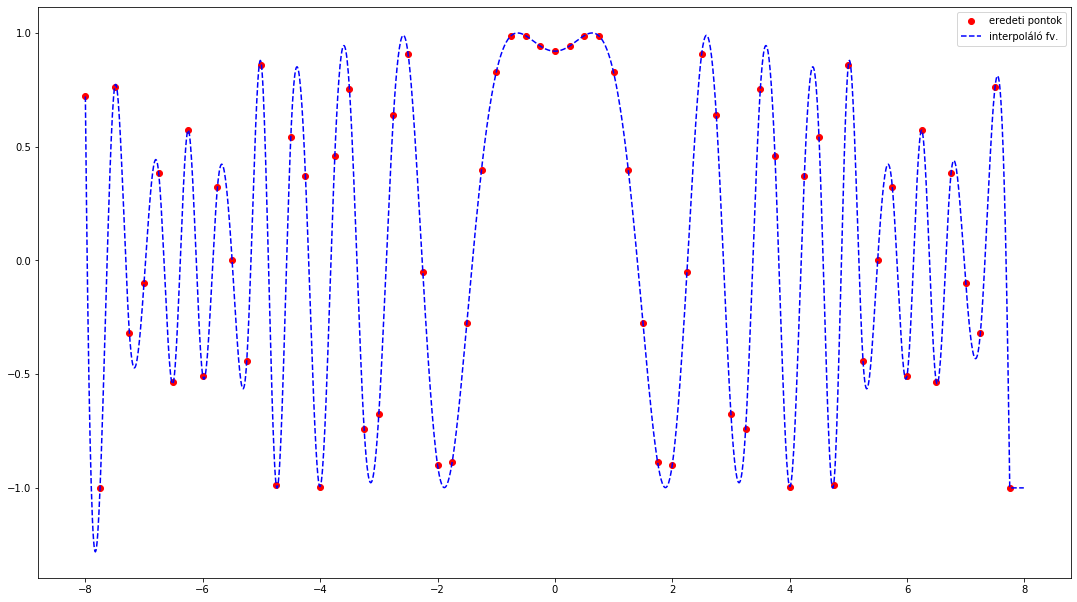
\includegraphics[width=\textwidth]{img/cubic.png}
\caption{Példa az \texttt{interp2d} használatára és eredményének megjelenítésére.}
\label{fig:cubic}
\end{figure}
    
    További egyszerűen használható függvény a numpy csomagban található
\texttt{interp1d}. Az \texttt{interp1d} esetében meg kell adni az \(x\)
és \(y\) értékeinket illetve egy olyan intervallumot az \([a, b]\)
intervallumon ami több alpontot tartalmaz. A megadott alpontok számától
függ a pontosság tehát lehetőleg elég sokat adjunk meg. Az
\texttt{interp1d} szakaszokra ad meg lineáris interpolácót. Ennek használata látható a következő kódpéldában.
\begin{python}
import numpy as np
import matplotlib.pyplot as plt
from matplotlib.pyplot import figure

x = np.linspace(0, 10, num=7, endpoint=True)
y = np.cos(-x**2 / 12)
xnew1 = np.linspace(0, 10, num=10, endpoint=True)
xnew2 = np.linspace(0, 10, num=20, endpoint=True)
xnew3 = np.linspace(0, 10, num=40, endpoint=True)
xnew4 = np.linspace(0, 10, num=80, endpoint=True)
yinterp1 = np.interp(xnew1, x, y)
yinterp2 = np.interp(xnew2, x, y)
yinterp3 = np.interp(xnew3, x, y)
yinterp4 = np.interp(xnew4, x, y)

plt.figure(figsize=(18.5, 10.5))
plt.plot(x, y, 'o',
    xnew1, yinterp1, '--',
    xnew2, yinterp2, '--',
    xnew3, yinterp3, '--',
    xnew4, yinterp4, '--')
plt.legend([
    "eredeti pontok",
    "interpolacio (10 db alpont)",
    "interpolacio (20 db alpont)",
    "interpolacio (40 db alpont)", 
    "interpolacio (80 db alpont)"])
plt.show()
\end{python}
A kimenete \aref{fig:interpolate3}. ábrán látható.

\begin{figure}[h!]
\centering
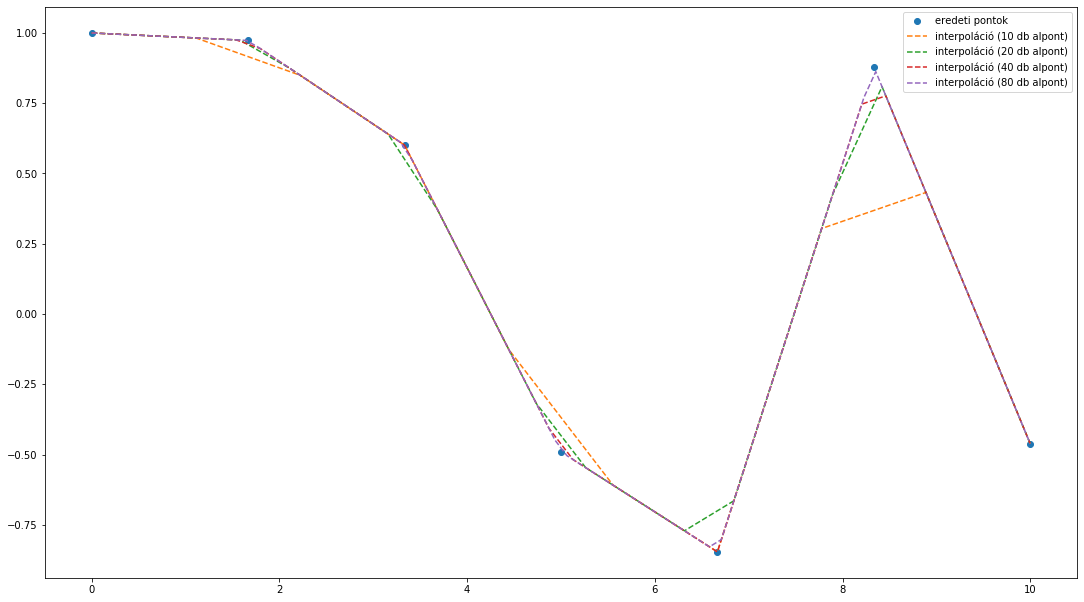
\includegraphics[width=\textwidth]{img/interpolate3.png}
\caption{Példa az \texttt{interp1d} használatára és eredményének megjelenítésére.}
\label{fig:interpolate3}
\end{figure}

\SubSection{Lagrange interpoláció}

    Legyenek a \(\phi_i\) bázisfüggvények a következők
\(\phi_1=1, \phi_2=x, \dots , \phi_n=x^{n-1}\) és legyenek
\(x_1, x_2,\dots, x_n\) alpontjaink és \(y_i=f(x_i)\) az alpontokhoz
tartozó függvény értékek. Ekkor a feladatunk az, hogy határozzuk meg a
legfeljebb n-1-ed fokú \(p\) polinomot amelyre igaz, hogy
\(p(x_i) = y_i\). Ez tulajdonképpen az alapfeladat a lényegi rész az, hogy
ezt a \(p\) polinomot hogyan állítjuk elő. A Lagrange féle előállítás a
következőképpen néz ki:
    \[
l_i(x)=\prod_{k=1, k\neq i}^n\frac{x-x_k}{x_i-x_k},
\]
majd ezekhez az \(l_i\) értékeket megszorozzuk a \(y_i\) értékeket és
megkapjuk a \(p\) polinomot
\[
p(x)=\sum_{i=1}^n y_il_i(x).
\]
Ezáltal meg kapjuk az \(f(x)\) függvényünk közelítését a \(p(x)\)
polinom által (\(f(x) \approx p(x)\)).

    Pythonban a \texttt{scipy.interpolate} csomag \texttt{lagrange} függvényével
tudunk a lagrange interpolációt számolni. Figyelni kell arra, hogy egy \texttt{poly}
nevű változóba tér vissza.
\begin{python}
import numpy as np
from scipy.interpolate import lagrange

import matplotlib.pyplot as plt
from matplotlib.pyplot import figure

x = np.linspace(0, 30, num=20, endpoint=True)
y = x**3
poly=lagrange(x,y)
xnew1 = np.linspace(0, 30, num=2, endpoint=True)
xnew2 = np.linspace(0, 30, num=4, endpoint=True)
xnew3 = np.linspace(0, 30, num=6, endpoint=True)
xnew4 = np.linspace(0, 30, num=8, endpoint=True)
xnew5 = np.linspace(0, 30, num=10, endpoint=True)

plt.figure(figsize=(18.5, 10.5))
plt.plot(x, y, 'o',
    xnew1, poly(xnew1), '--',
    xnew2, poly(xnew2), '--',
    xnew3, poly(xnew3), '--',
    xnew4, poly(xnew4), '--',
    xnew5, poly(xnew5), '--')
plt.legend([
    "eredeti pontok",
    "interpolacio (2 db alpont)",
    "interpolacio (4 db alpont)",
    "interpolacio (6 db alpont)",
    "interpolacio (8 db alpont)",
    "interpolacio (10 db alpont)"])
plt.show()
\end{python}
A program futásának eredménye \aref{fig:lagrange}. ábrán látható.

\begin{figure}[h!]
\centering
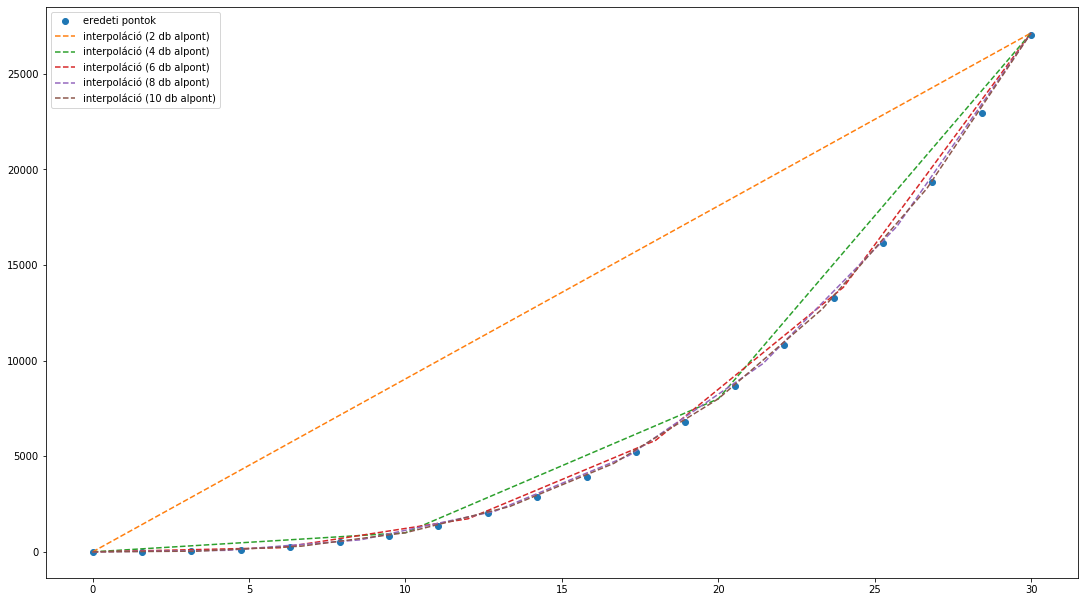
\includegraphics[width=\textwidth]{img/lagrange.png}
\caption{Példa a Lagrange interpolációra.}
\label{fig:lagrange}
\end{figure}
    
    Látszik, hogy a pontosság itt is függ a megadott alpontok számától. Bár a
Lagrange interpolációnak létezik Python-os implementációja , numerikusan
instabil ezért ha mindenféleképpen ezt szeretnénk használni, érdemesebb a
saját implementációnkat elkészíteni.

\SubSection{Spline interpoláció}

    Spline interpoláció esetén is megvannak az \(x_i\) pontjaink és \(y_i\)
függvényértékeink, és ezek mellett keressük azt az \(S(x)\) függvényt,
mely teljesíti az alábbi feltételeket:
\begin{align*}
S(x) &= S_i(x), &x\in[x_i, x_{i+1}],\\
S(x_i) &= y_i, &(i=1, \dots, n),\\
S_i(x_{i+1}) &= S_{i+1}(x_{i+1}), &(i=1, \dots, n-2).
\end{align*}
    Az első feltétel megfogalmazza, hogy szakaszokból áll a függvényünk, a
második megmondja, hogy valóban interpoláló függvény az \(S(x)\)
függvényünk, és a harmadikkal a folytonosság van definiálva az \([a, b]\)
intervallumon.

    A spline meghatározásánál felírunk \(n\) darab \(k\)-ad fokú polinomot.
Ebből látszik, hogy az ismeretlenek száma \(n(k + 1)\). Az első és a
harmadik feltételből következik az, hogy a feltételek száma
\((k+1)n-(k-1)\), ugyanis \(k-1\) db simasági feltétel a \(n-1\) belső
pontban ebből jön az, hogy \((n-1)(k-1)\) és \(2n\) interpolációs
feltétel. Összesen \((n-1)(k-1)+2n=(k+1)n-(k-1)\), és ebből látszik, hogy
hiányzik a spline egyértelműségéhez még \(k-1\) darab feltétel. Ezeket a
végpontokra szokták megadni.

    Vegyük először a lineáris spline interpolációt ebben az esetben a
\(k=1\), és a három feltétel egyértelműen meghatározza. Minden
\([x_k, x_{k+1}]\) intervallumon:
\begin{align*}
S_k(x_k) &= a_kx_k+b_k=y_k \\
S_k(x_{k+1}) &= a_kx_{k+1}+b_k=y_{k+1}.
\end{align*}
Ebből a kétismeretlenes egyenletrendszerből meghatározható \(a_k\) és
\(b_k\).

    Beszélhetünk még kvadratikus splineokról is. Ekkor a \(k=2\) és
\(k-1 = 1\) feltétel hiányzik a spline egyértelmű felírásához. Ezt a
feltételt általában az intervallum elején vagy végén a derivált
megadásával szokás teljesíteni. Az így felvázolt esetben az egymás
melletti intervallumokra Hermite interpolációt alkalmazva meghatározható
a spline.

    Gyakorlatban azonban a harmadfokú spline interpolációt használjuk
túlnmyómó részt, és csak harmadfokú splineról beszélünk, viszont ezek
további feltételek felírását követelik meg, úgy mint:
\begin{align*}
S_i'(x_{i+1}) &= S_{i+1}'(x_{i+1}), &(i=1, \dots, n-2),\\
S_i''(x_{i+1}) &= S_{i+1}''(x_{i+1}), &(i=1, \dots, n-2),\\
S''(x_{1}) &= A_n \quad \textrm{és}, &S''(x_{n}) = B_n
\end{align*}

    Pythonban használhatjuk a harmadfokú spline-t is. Ehhez elő kell készíteni az értékeket
a \texttt{scipy.interpolate} csomagban megtalálható \texttt{splprep} függvénnyel,
majd utána tudjuk használni a \texttt{splev} függvényt, amely a harmadfokú
spline-t adja vissza.

    Először vegyünk egy függvényt és pár alpontot. Legyen most ez a szinusz
függvény és próbáljuk ezt közelíteni spline-al!
\begin{python}
import numpy as np
import matplotlib.pyplot as plt
from scipy import interpolate
from matplotlib.pyplot import figure


x = np.arange(0, 2*np.pi+np.pi/4, 2*np.pi/8)
y = np.sin(x)
tck = interpolate.splrep(x, y, s=0)
xnew = np.arange(0, 2*np.pi, np.pi/50)
ynew = interpolate.splev(xnew, tck, der=0)

plt.figure(figsize=(18.5, 10.5))
plt.plot(x, y, '-x', xnew, ynew, 'g--')
plt.legend(['sin(x) adott pontokra', 'harmadfoku spline'])
plt.axis([-0.05, 6.33, -1.05, 1.05])
plt.show()
\end{python}

\begin{figure}[h!]
\centering
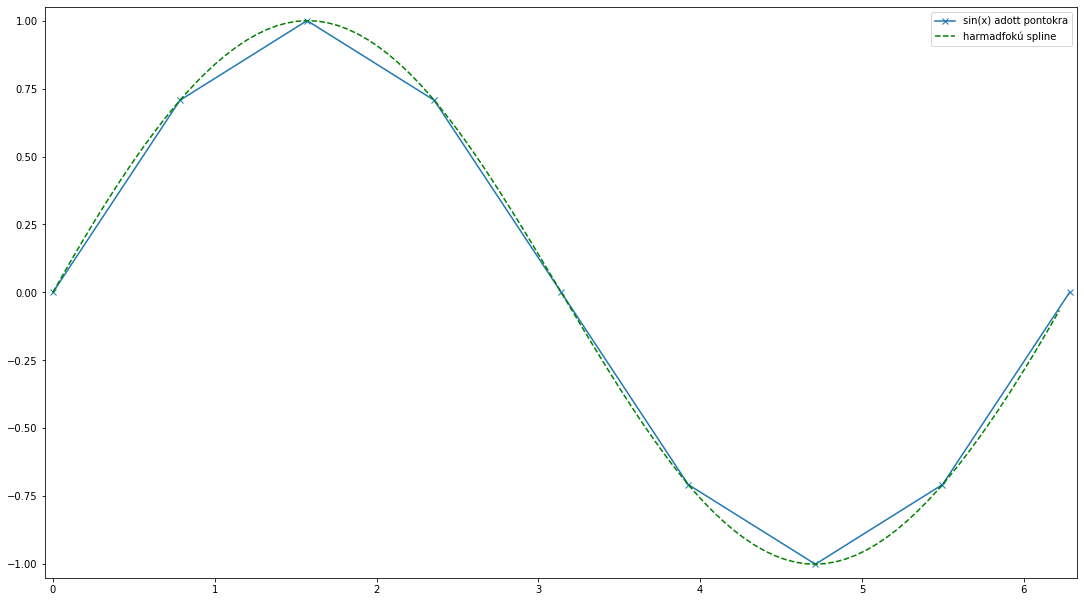
\includegraphics[width=\textwidth]{img/spline.png}
\caption{Példa spline segítségével történő interpolációra.}
\label{fig:spline}
\end{figure}

\Aref{fig:spline}. ábrán látható, hogy a harmadfokó spline jól közelíti a függvényünket, hiszen
nagyjából lefedi, és a megadott pontokban felveszi a megadott
értékeket.

\SubSection{Hermite interpoláció}

    A harmadik interpoláció amit csak megemlítek, az a Hermite interpoláció.
Hermite interpoláció esetén ugyan szintén megvannak az
\(x_0, x_1, \dots, x_n \in [a,b])\) pontjaink, mint eddig és vannak
mellé $m\_0, m\_1, \dots, m\_k \quad (k\leq n)$ multiplicitások is
úgy, hogy $\sum_{i=0}^k m_i=n+1$, továbbá adottak az
\[
f^{(j)}(xi)=y_{ij}, \quad (i=0,\dots,k \quad \textrm{és}\quad j=0,\dots,m-1)
\]
értékek is. Feladatunk az, hogy megkeressünk egy $n$-ed fokú $P$ polinomot
melyre igaz hogy:
\[
P^{(j)}(xi)=y_{ij}, \quad (i=0,\dots,k \quad\textrm{és}\quad j=0,\dots,m-1).
\]

\Section{Sajátérték, sajátvektor számítása}

    A mátrixok sajátértékéhez és sajátvektorához szükségünk lehet a komplex
számok halmazára is. Egy ilyen komplex számokból álló mátrixot a valós
számokból állóhoz hasonlóan \(\mathbb{C}^{mxn}\)- el jelöljük
\((\mathbb{R}^{mxn} \subset \mathbb{C}^{mxn})\). Nézzük először a
sajátvektor és a sajátérték definícióját!

Legyen \(A \in \mathbb{C}^{nxn}\) tetszőleges mátrix. A
\(\lambda \in \mathbb{C}\) számot az \(A\) mátrix sajátértékének és az
\(x \in \mathbb{C}^n \quad (x\neq0)\) vektort pedig \(\lambda\)
sajátértékhez tartozó sajátvektornak nevezzük, ha
\[
Ax=\lambda x.
\]
    Fontos, hogy egy mátrix sajátértékeinek összeségét a mátrix spektrumának
nevezzük és a spektrumból a mátrix fontos tulajdonságait lehet kiolvasni
például az alábbiakat.
\begin{itemize}
\item Egy négyzetes mátrix akkor és csak akkor nemszinguláris ha
egyik sajátértéke sem nulla.
\item Egy mátrix akkor és csak akkor pozitív
definit, ha minden sajátértéke pozitív.
\end{itemize}

    A sajátértékeket úgy kaphatjuk meg, ha megoldjuk a karakterisztikus
egyenletet amely a következő:
\[
\phi(\lambda) = det(A-\lambda i) = 0.
\]
Ezt kifejtve megkapjuk a \(\lambda\) változó \(n\)-ed fokú polinomját, azaz a:
\[
\phi(\lambda)=(-1)^n\lambda^n+p_{n-1}\lambda^{n-1}+\dots+p_1\lambda+p_0
\]
karakterisztikus polinomot. Komplex számok körében ennek a polinomnak
pontosan \(n\) darab zérushelye van, tehát egy \(A\in \mathbb{C}^{nxn}\)
mátrixnak pontosan \(n\) darab sajátértéke van, ha figyelembe vesszük a
multiplicitásokat.

    Most térjünk rá a Python-ban való megvalósítására! A sajátértékeket és
vektorokat a \texttt{numpy.linalg} csomagban található \texttt{eig} metódussal
tudjuk kiszámolni az alábbi módon.
\begin{python}
from numpy import linalg as LA
import numpy as np

A = np.random.randint(10, size=16)
A = np.reshape(A,(4,4))

w, v = LA.eig(A)
print("Sajatertekek:\n")
print(w)
print("\nSajatvektorok:\n")
print(v)
\end{python}
    Az \texttt{eig} egy \(n \times n\)-es mátrixot vár és két vektorral tér vissza
az első (\texttt{w}) tartalmazza a sajátértékeket, a második (v) pedig a saját
vektorokat normalizát alakban. Az $i$-edik (\texttt{w[i]}) sajátértékhez az
$i$-edik (\texttt{v[:, i]}) a oszlop tartalmazza a sajátvektort.

    A \texttt{numpy.linalg} csomagban találunk még egy \texttt{eigvals} függvényt, mely csak a
sajátértékeket számolja ki, és ugyanúgy egy \(n \times n\)-es mátrixot vár
paraméterként.
\begin{python}
w = LA.eigvals(A)
print("Sajatertekek:\n")
print(w)
\end{python}
Ezek a metódusok a \texttt{\_geev} LAPACK rutint használják.

\Section{Legkisebb négyzetek módszere}

Nézzünk meg egy példát a legkissebb négyzetek módszerének szemléltetésére Python segítségével!

Legyen a feladatunk az, hogy kapott mérési eredményekre ráillesszünk egy
egyenest! Adottak a mért értékek \(y \in R^n\) és a hozzájuk tartozó
helyek $x\in R^n$. Ezek alapján keressük a \(y= a_0+a_1x\)
egyenest melyre a
\[
\sum_{i=0}^N
[y_i - (a_0 + a_1 x_i)]^2
\]
minimális. Szerencsénkre erre is tartalmaz beépített metódust a
\texttt{NumPy}. A \texttt{linalg} csomagban található \texttt{lstsq}
metódus megadja az egyenest amire szükségünk van:
\begin{python}
import numpy as np
import matplotlib.pyplot as plt
from matplotlib.pyplot import figure 

x = np.array([0, 1, 2, 3, 4, 5, 6, 7, 8])
y = np.array([-1, 0.2, 0.9, 2.1, 3.2, 3.8, 4.0, 4.3, 4.8])
a = np.vstack([x, np.ones(len(x))]).T

m, c = np.linalg.lstsq(a, y, rcond=None)[0]

plt.figure(figsize=(18.5, 10.5), dpi=150)
plot = plt.plot(x, y, 'o', label='Eredeti adataink', markersize=10)
plot = plt.plot(x, m*x + c, 'r', label='Illesztett egyenes')
plot = plt.legend()
plt.show(plot)
\end{python}
A program futásának eredménye \aref{fig:lsqt}. ábrán tekinthető meg.

\begin{figure}[h!]
\centering
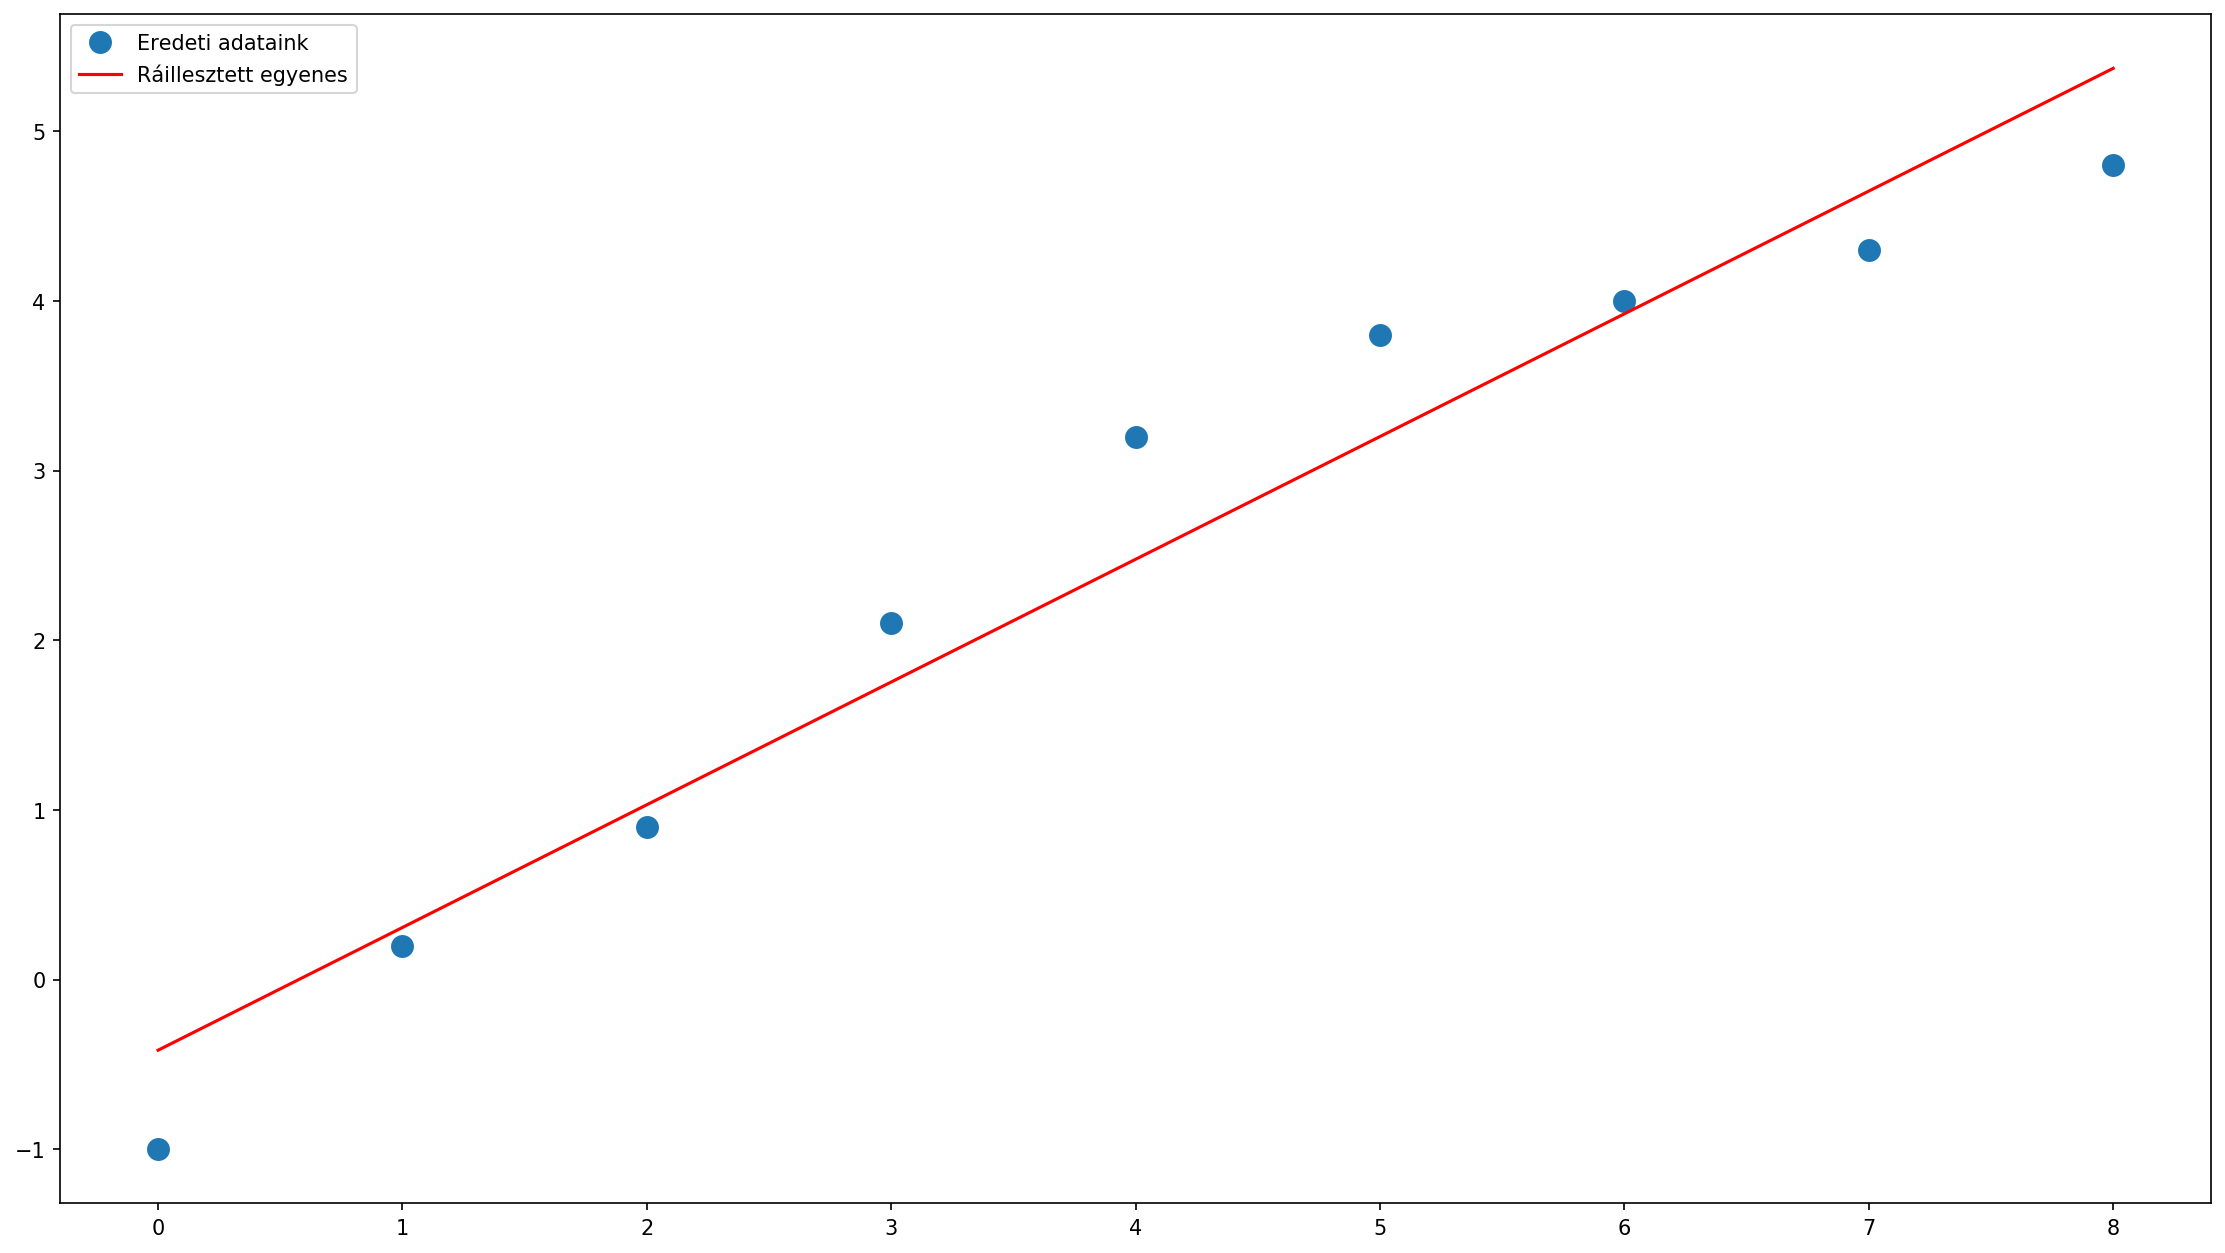
\includegraphics[width=\textwidth]{img/lsqt.png}
\caption{A legkisebb négyzetek módszerének szemléltetése.}
\label{fig:lsqt}
\end{figure}
    
\Section{Numerikus deriválás}

A numerikus deriválás alapfeladata az, hogy az analítikusan ismeretlen,
vagy nehezen számolható, esetleg csak diszkrét pontokban ismert
\(f: D(\subseteq \mathbb{R})\rightarrow \mathbb{R}\) függvény
deriváltját közelítsük adott pontokban.

Többféleképpen indulhatunk neki. Készíthetünk például egy interpolációt, mely
közelít az \(f\) függvényünkhöz, és akkor az interpolációnk \(k\)-adik
deriváltja fog közelíteni az \(f\) függvényünk \(k\)-adik
deriváltjához.

Ha \(f \in C^2[a,b]\), akkor felírhatjuk rá a másodfokú Taylor polinomot,
amiből kifejezhetjük az alábbi összefüggést:
\[
f'(x)\approx \frac{f(x+h)-f(x)}{h},
\]
melynek hibája \(O(h)\). A harmadfokú Taylor polinommal még pontosabb
közelítést kaphatunk:
\[
f'(x)\approx \frac{f(x+h)-f(x-h)}{2h}.
\]
Másodfokú deriváltra alkalmazhatjuk az alábbi összefüggéseket:
\[
f''(x)\approx \frac{f(x)-2f(x+h)+f(x+2h)}{h^2},
\]
\[
f''(x)\approx \frac{f(x+h)-2f(x)+f(x-h)}{h^2}.
\]
A második képlet a centrális differencia formula. Mind a két képlet
hibája \(O(h^2)\).

Ezek a következő formában implementálhatók Python-ban:
\begin{python}
import numpy as np
import matplotlib.pyplot as plt

def f(x):
    return x**2 + x**3 + 3

def firstDerivate1(x, h):
    return (f(x + h) - f(x)) / h

def firstDerivate2(x, h):
    return (f(x + h) - f(x - h)) / 2*h

def secondDerivate1(x, h):
    return (f(x) - 2*f(x + h) + f(x + 2*h)) / h*h

def secondDerivate2(x, h):
    return (f(x + h) - 2*f(x) + f(x - h)) / h*h
\end{python}
Polinom segítségével megadott pontokkal a módszert \aref{fig:deriv}. ábrán látható formában szemléltethetjük.

\begin{figure}[h!]
\centering
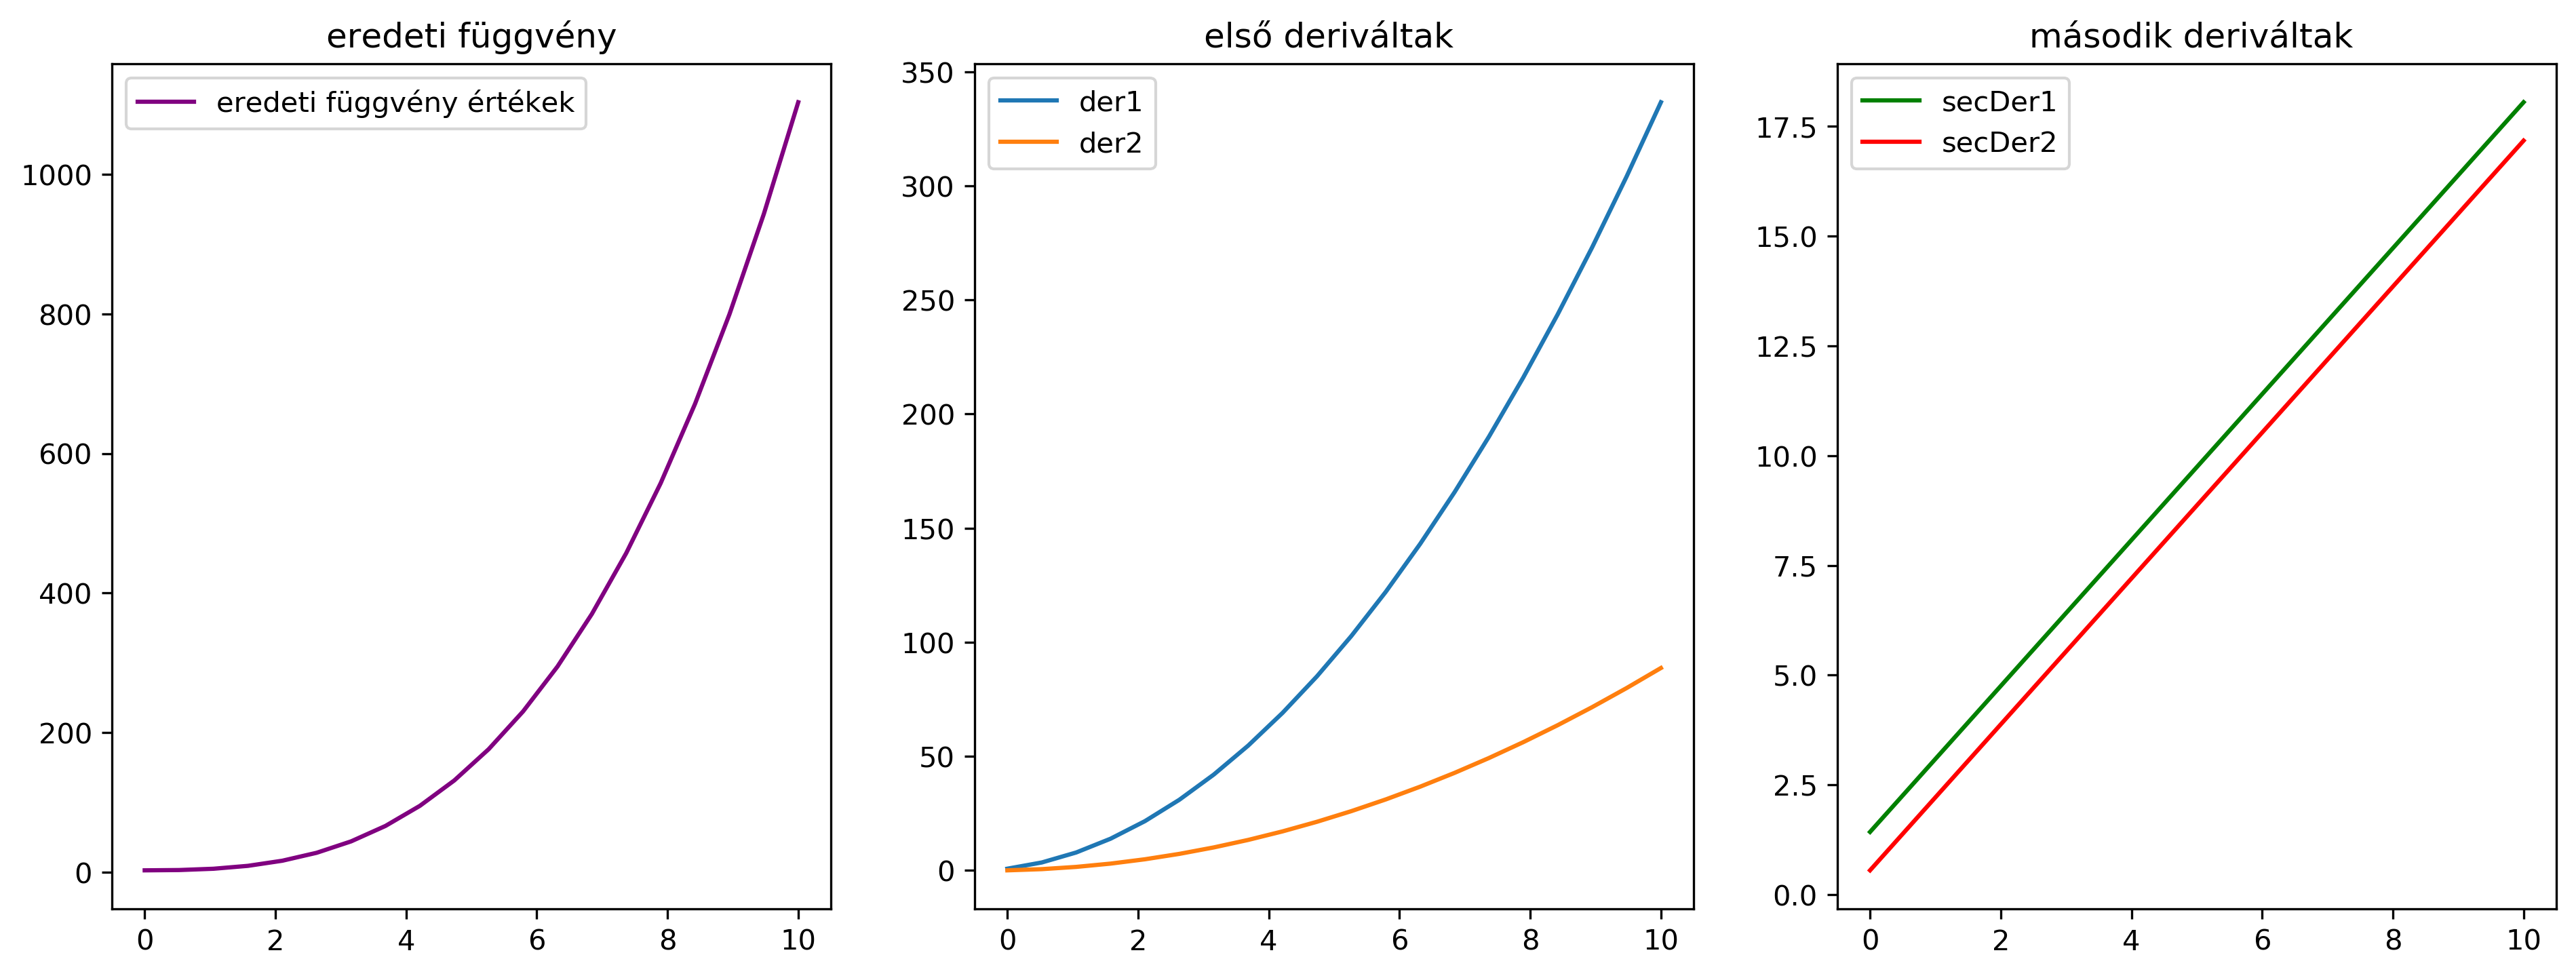
\includegraphics[width=\textwidth]{img/deriv.png}
\caption{A numerikus deriválás szemléltetése.}
\label{fig:deriv}
\end{figure}
    
    Interpolációkkal való közelítéshez használható többek között a Newton, Lagrange és a
Spline interpoláció is.

\Section{Numerikus integrálás}

    Numerikus integrálásnál a Newton-Leibnitz formulából indulunk ki. Ha
adott egy \(f\) függvény és az Riemann integrálható \([a, b]\)-n, és itt
létezik primitív függvénye, akkor
\[
I = \int^b_a f(x)dx = F(b) - F(a).
\]

Ezt a képletet viszont csak akkor tudjuk alkalmazni, ha létezik \(f\)-nek
primitív függvénye, egyébként numerikus integrálást kell alkalmaznunk.

Numerikus integrálást úgy tudunk alkalmazni, ha az \(f\) függvényünket
közelítjük egy \(p\) interpolációs polinommal, és ezáltal a határozott
integrál értékét általános formában közelíthetjük:
\[
I = \int_a^b f(x)w(x)dx \approx \int_a^b p(x)w(x)dx,
\]
ahol $w(x) \geq 0$ egy tetszőleges súlyfüggvény.

    Integráláshoz találunk előre megírt függvényeket a \texttt{scipy.integrate}
csomagban a \texttt{quad}, \texttt{dblquad}, \texttt{tplquad} formájában. A \texttt{quad} egy általános esetekben használható függvény, a
\texttt{dblquad} a \texttt{quad}-hoz hasonló de kétszeres integrálást
végez, míg a \texttt{tplquad} pedig háromszorosan integrál.
Az alábbi példában szereplő módon használható:
\begin{python}
import scipy.integrate as integrate

def f(x):
    return x + x**2 + 3

x = np.linspace(0, 10, num=20)
y = x**2 + x**3 + 3    
result = integrate.quad(f, 0, 10)
\end{python}

    Vannak természetesen egyébb algoritmusok is, melyeket lehet használni, ilyen a
Lagrange formula vagy a zárt vagy nyitott Newton-Cotes formulák is. Ezek
mellett ott vannak még a téglalap és trapéz formulák. A Newton-Cotes
formulákra visszavezethető a Simpson és az érintő formula is.

    Nézzük meg ezek közül először a két legegyszerűbbet a téglalap
formulákat és a trapéz módszert. Kezdjük a téglalap formulákkal!

Az
\(f\) függvény integrálját szeretnénk az \([a ,b]\) intervallumon meghatározni. Legyen
\(h=(b - a)/n\) a lépésköz ekkor az első téglalap formula a következő:
\[
I^{(1)}= h  \sum^{n-1}_{j=0}y_j,
\]
a második pedig:
\[
I^{(2)}= h  \sum^{n}_{j=1}y_j,
\]
és van egy harmadik is:
\[
I^{(3)}= h  \sum^{n}_{j=1}y_{j-1/2}.
\]
Látszik hogy a formulák a téglalapokat illesztenek a függvényre és ezek
területének az összege adja meg az integrál értékét.
Ezek Python implementációja például az alábbi lehet:
\begin{python}
def teglalap1(x, h, n):
    ossz = 0
    for i in range(0, n-1):
        ossz = ossz + f(x[i])
    return h * ossz

def teglalap2(x, h, n):
    ossz = 0
    for i in range(1, n):
        ossz = ossz + f(x[i])
    return h * ossz

def teglalap3(x, h, n):
    ossz = 0
    for i in range(1, n):
        x1 = (x[i-1] + x[i]) / 2
        ossz = ossz + f(x1)
    return h * ossz
\end{python}    
    Ezek nem ugyanazt az eredményt adják, de elég sok alpont esetén
az egzakt megoldáshoz tartanak. A téglalap formula hibája az alpontok
számától függ lineárisan, azaz \(O(h)\).

    Most nézzük a Trapéz módszert! A trapéz módszernek van egy egyszerű és
egy összetett változata is. Először vegyük az egyszerűt. Ebben az
esetben 1 alpontunk van tehát \(h=1\). Legyen \(a=x_0\) és \(b=x_1\)
ekkor: \[
\int^b_a f(x)dx \approx \frac{y_0+y_1}{2}h.
\]
A számítás az adott intervallumra az alábbi:
\begin{python}
def trapez_egyszeru(x, a, b, h):  
    return (f(a) + f(b)/2) * h
\end{python}
    Ez az esetek jelentős részében nem ad eléggé pontos eredményt. most nézzük meg az összetett trapéz
módszert.

Az Összetett trapéz módszer esetén már több alpontuk van tehát
\(h\geq 1\) és az alábbi képletet alkalmazzuk:
\[
\int^b_a f(x)dx \approx \sum^{n-1}_{j=0}\frac{x_{i+1}-x_i}{2}(y_i+y_{i+1}).
\]
A hozzá tartozó Python implementáció a következő:
\begin{python}
def trapez_osszetett(x, n):
    ossz = 0
    for i in range(0, n-1):
        xi = (x[i+1] - x[i]) / 2
        ossz = ossz + xi * (f(x[i]) + f(x[i+1]))
    return ossz
\end{python}
    Ez már sokkal pontosabb eredményt ad, mint az egyszerű trapéz
módszer.

    Folytassuk az érintő formulával! Az érintő formula egy nyílt
Newton-Cotes formula melyre:
\[
\int^b_a f(x)dx \approx (b-a)f\left( \frac{a+b}{2}\right)
\]
Ez a formula úgy is értelmezhtő, hogy az \(f\) függvényünket a
középpontjához húzott egyenessel közelítjük az \([a, b]\) intervallumon,
és az egyenes alatti területet vesszük. Ebből következik, hogy maximum
első fokú polinomig pontos. Gyakorlatban nem ezt a képletet szokták
alkalmazni, hanem az intervallumot felosztják n egyenlő részre és a következő
képletet alkalmazzák:
\[
\int^b_a f(x)dx \approx \frac{(b-a)}{n}\sum^{n}_{i=1}f\left( a-\frac{h}{2}+ih\right)
\]
Nézzük meg ezek implementációját!
\begin{python}
def erinto_egyszeru(x, a, b):  
    return (b - a) * (f(b + a) / 2)

def erinto_osszetett(x, a, b, n, h):
    d = (b - a) / n
    ossz = 0
    for i in range(1, n):
        xi = a - (h / 2) + (i * h)
        ossz = ossz + f(xi)
    return ossz * d
\end{python}
Az egyszerű érintő formula hiba becslése:
\[
\left| \int^a_b f(x)dx-(b-a) f \left( \frac{a+b}{2} \right)\right| \leq \frac {(b-a)^3M_2}{24}.
\]

    Végül jöjjön a Simpson formula mely egy zárt Newton-Coats formula, melyre
\(n=2\). Ennek is van egyszerű és összetett alakja. Az egyszerű alakhoz
3 alpontra van szükségünk \(x_1=a, x_1=\frac {a+b}{2}, x_2=b\) és
alakalmazzuk a három pontra támaszkodó Lagrange-féle interpolációs
polinomot:
\[
\int^b_a f(x)dx \approx \frac{b-a}{6} \left[f(a)+4f\left(\frac{a+b}{2}\right)+f(b)\right].
\]

Az összetett Simpson formula esetén is az intervallumot felosztjuk \(n\)
egyenlő részre, és akkor ilyen módon változik meg a képletünk:
\[
\int^b_a f(x)dx \approx \sum^{n-1}_{i=0}\frac{x_{i+1}-x_i}{6}
\left[
f(x_i) + 4f\left( \frac{x_i+x_{i+1}}{2}\right)+ f({x_{i+1}})
\right].
\]
Ezeknek az implementációja az alábbi:
\begin{python}
def simpson_egyszeru(x, a, b):  
    return ((b-a)/6) * (f(a)+ 4*f((a+b)/2)+f(b)) 
    
def simpson_osszetett(x, n):
    ossz = 0
    for i in range(0,n-1):
        x1 = (x[i+1]-x[i])/6
        x2 = (f(x[i])+ 4*f((x[i]+x[i+1])/2)+f(x[i+1]))
        ossz = ossz + (x1*x2)
    return ossz
\end{python}
A Simpson formula hibája:
\[
\left|\int^a_b f(x)dx- S_n(f)\right| \leq \frac {M_4(b-a)}{32 \cdot 90}h^4 = \frac {M_4(b-a)^5}{2880n^4}.
\]
